\chapter{Алгоритмы}

\begin{multicols}{2}
    \raggedcolumns

    \section{Анализ алгоритмов. Понятие о сложности по времени и по памяти. Асимптотика, О-
    символика. Доказательство корректности алгоритмов.}
    \begin{definition}{(O-нотация)}{}
        Пусть $f,g: \ \N \to \N$. Тогда $f = \bigOO(g)$, если $\exists C > 0$ и $\exists N: \ \forall n > N$:
        \[
            f(x) \leq Cg(x)  
        \]
    \end{definition}
    \begin{proposition}{}{}
        $f = \bigOO(g) \Leftrightarrow \exists C > 0 \ \forall n \in \N: \ f(n) \leq Cg(n).$
    \end{proposition}
    \begin{definition}{}{}
        $f, g: \ \N \to\N$. Тогда $f = \Omega(g)$ или $g = \bigOO(f)$ или $\exists C > 0\ f(n) \geq Cg(n).$
    \end{definition}
    \begin{definition}{}{}
        $f = \Theta (g)$, если $f = \bigOO(g)$ и $g = \bigOO(f)$ или $\exists C_1, C_2 > 0\ \forall n \in \N C_1 g(n) \leq f(n) \leq C_2g(n)$.
    \end{definition}
     Примеры:
     \begin{multicols}{2}
        \begin{itemize}
            \item $n = \bigOO(n^2), \ \mathmbox{n^2 = \Omega(n);}$
            \item $n\log n = \bigOO(n^2)$;
            \item $3n + n^2 = \Theta(n^2)$;
            \item $\log^{10} n = \bigOO(n^{1/5}).$
        \end{itemize}
     \end{multicols}
     \begin{theorema}{(Мастер Теорема)}{}
        Пусть $T(n)$ -- время работы какого-то алгоритма на входе длины $n$, причем $T(n) = aT(\dfrac{n}{b}) + f(n)$. Тогда 
        \begin{enumerate*}
            \item Если $\exists \varepsilon > 0: \ f(n) = \bigOO(n^{\log_ba - \varepsilon})$, то \[
                T(n) = \Theta(n^{log_ba})  
            \]
            \item Если $f(n) = \Theta (n^{\log_ba})$, то 
            \[
                T(n) = \Theta (n^{log_ba}\cdot \log n)
            \]
            \item Если $\exists \varepsilon > 0: \ f(n) = \Omega(n^{\log_ba + \varepsilon})$, причем $\exists c<1: \ \mathmbox{a\cdot f^{n/b} \leq c\cdot f(n)}$, ($\forall n$, начиная с некоторого), то $T(n) = \Theta (f(n))$.
        \end{enumerate*}
     \end{theorema}
     \cons Пусть $T(n) = 2T(n/2) + \Theta(n)$. Тогда $T(n) = \Theta(n\log n)$.
     \par
     \myexe{Префиксные суммы.} Пусть $a_1, \ldots, a_n$ -- статический массив. $l,r$ -- индексы. Сообщить $a_l + a_{l+1} + \ldots + a_r$
     \par
     \begin{itemize}
        \item[] Наивное решение: $\bigOO(n\cdot q)$, где $q$ -- количество запросов;
        \item[] Префиксные суммы:
        \begin{algorithmic}[1]
            \State pref[$0$] = $0$
            \State pref[$i$] = $a_1 + \ldots + a_i$
            \State pref[$i+1$] = $a_1 + \ldots + a_i + a_{i+1}$
        \end{algorithmic}
        Это проходит за $\bigOO(n)$. Итого
        \[
            a_l + \ldots a_r = pref[r] - pref[l-1]  
        \]
        Решение $\bigOO(n+q)$
     \end{itemize}
     \myexe{Бинарный поиск} Отсортированный массив $a_1 \leq a_2 \leq \ldots \leq a_n$. Вопрос: есть ли $x$ в этом массиве.
     \begin{itemize}
        \item[] Наивное: $\bigOO(n\cdot q)$
        \item[] $\bigOO(q\cdot \log n + n)$
        Пусть $l=1, \ r=n$. $x$ лежит в отрезке $[l,r]$. Посмотрим на середину массива с индексом $m = \dfrac{l+r}{2}$. Тогда:
        \begin{enumerate*}
            \item Если $a[m]=x$ -- выдать да;
            \item Если $a[m] < x$, то ответ справа $l=m$, повторяем;
            \item Иначе $r=m$.
        \end{enumerate*}
        \begin{algorithmic}[1]
            \Repeat 
            \State int $m = \dfrac{(l+r)}{2}$
            \If  $a[m] == x$
            \State Выдать $yes$
            \ElsIf $a[m]<x$
            \State $l = m$
            \Else 
            \State $r=m$ 
            \EndIf
            \Until $(r-l>1)$
            \If ($a[l] == x || a[r] == x$)
            \State Выдать $yes$
            \Else
            \State Выдать $no$
            \EndIf
        \end{algorithmic}
     \end{itemize}
    \section{Строки и операции над ними. Представление строк. Вычисление длины, конкатенация.
    Алгоритмы поиска подстроки в строке.}

    \section{Сортировки. Нижняя теоретико-информационная оценка сложности задачи сортировки.
    Алгоритмы сортировки вставками, пузырьком, быстрая сортировка, сортировка
    слиянием. Оценка сложности.}
    \subsection*{Сортировки}
    Постановка задачи: Дан массив объектов $a_1,\ldots, a_n$. На объектах задано отношение порядка:
    \[
        \forall x,y, \hspace*{0.5cm} x < y \text{ или } x = y \text{ или } x > y
    \]  
    Цель: переставить элементы, чтобы они шли в порядке неубывания (невозрастания). Или также найти перестановку: $\sigma:\ [n] \to [n]$:
    \[
        a_{\sigma(1)} \leq a_{\sigma(2)} \leq \ldots \leq a_{\sigma(n)}  
    \]
    \begin{theorema}{}{}
        Любой алгоритм сортировки, основанный на сравнениях, требует $\Omega(n\log n)$ сравнений в худшем случае на массиве длины $n$. 
    \end{theorema}
    \begin{lemma}{}{}
        $\log (n!) = \Theta(n\log n)$
    \end{lemma}
    \subsubsection*{Сортировка слиянием}
    Сортировка за $\bigOO(n\log n)$, основанная на сравнениях.
    Разобьем массив на два равных куска:
    \begin{center}
        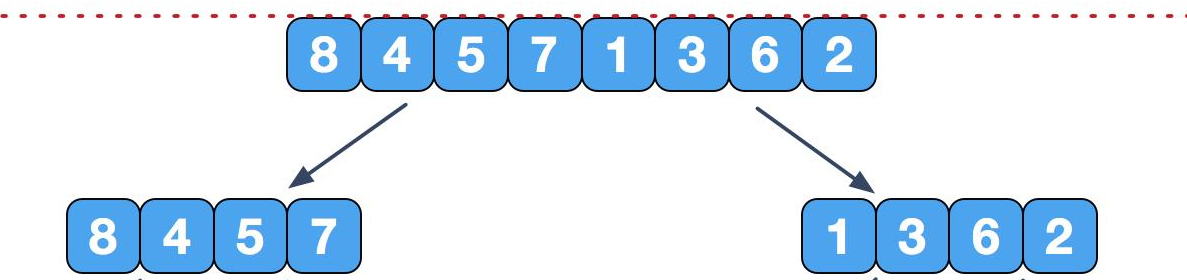
\includegraphics[scale=0.25]{images/1st_step.png}        
    \end{center}
    Рекурсивно продолжаем:
    \begin{center}
        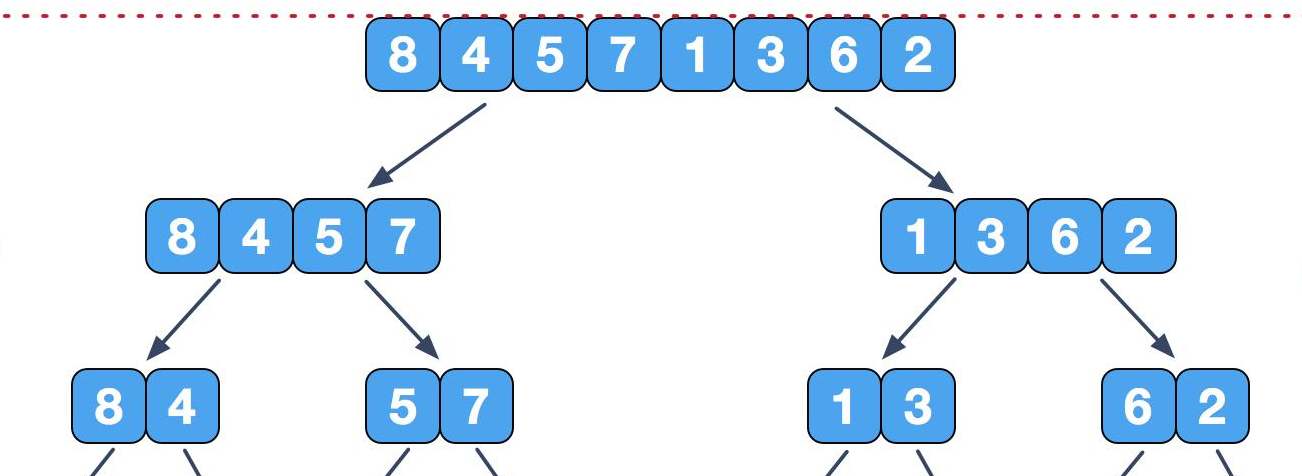
\includegraphics[scale=0.25]{images/2nd_step.png}
    \end{center}
    Следующий шаг:
    \begin{center}
        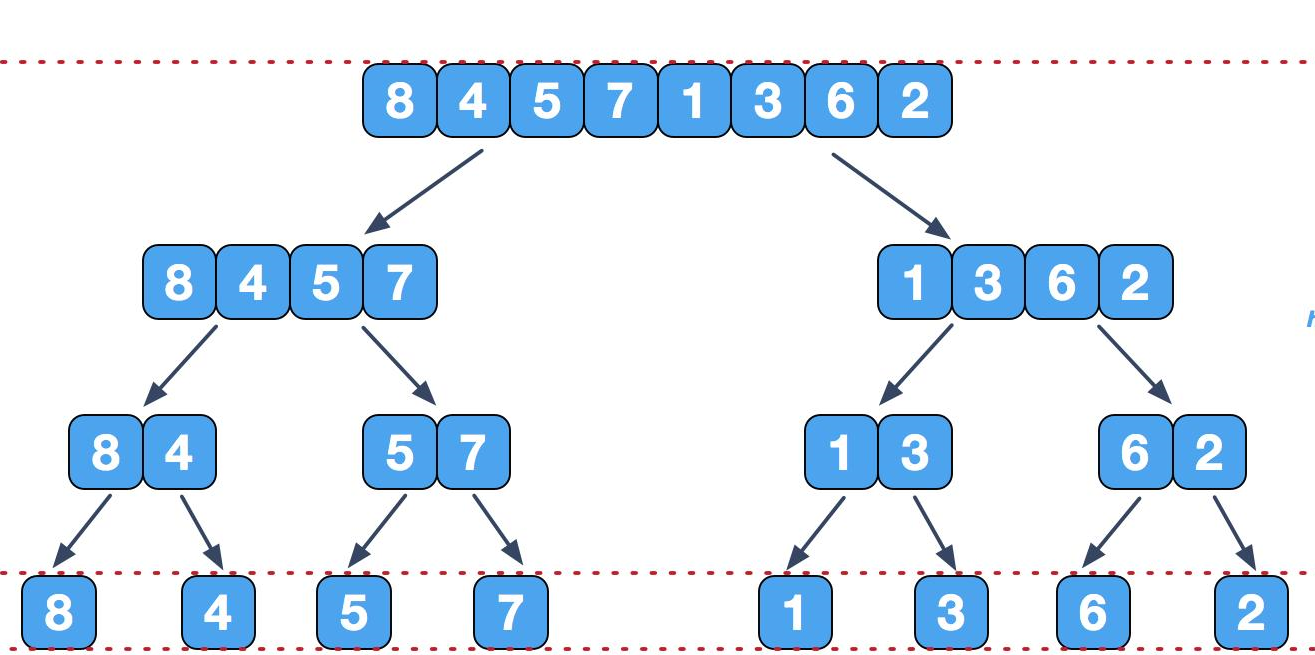
\includegraphics[scale=0.25]{images/3rd_step.png}
    \end{center}
    Сортируем полученное:
    \begin{center}
        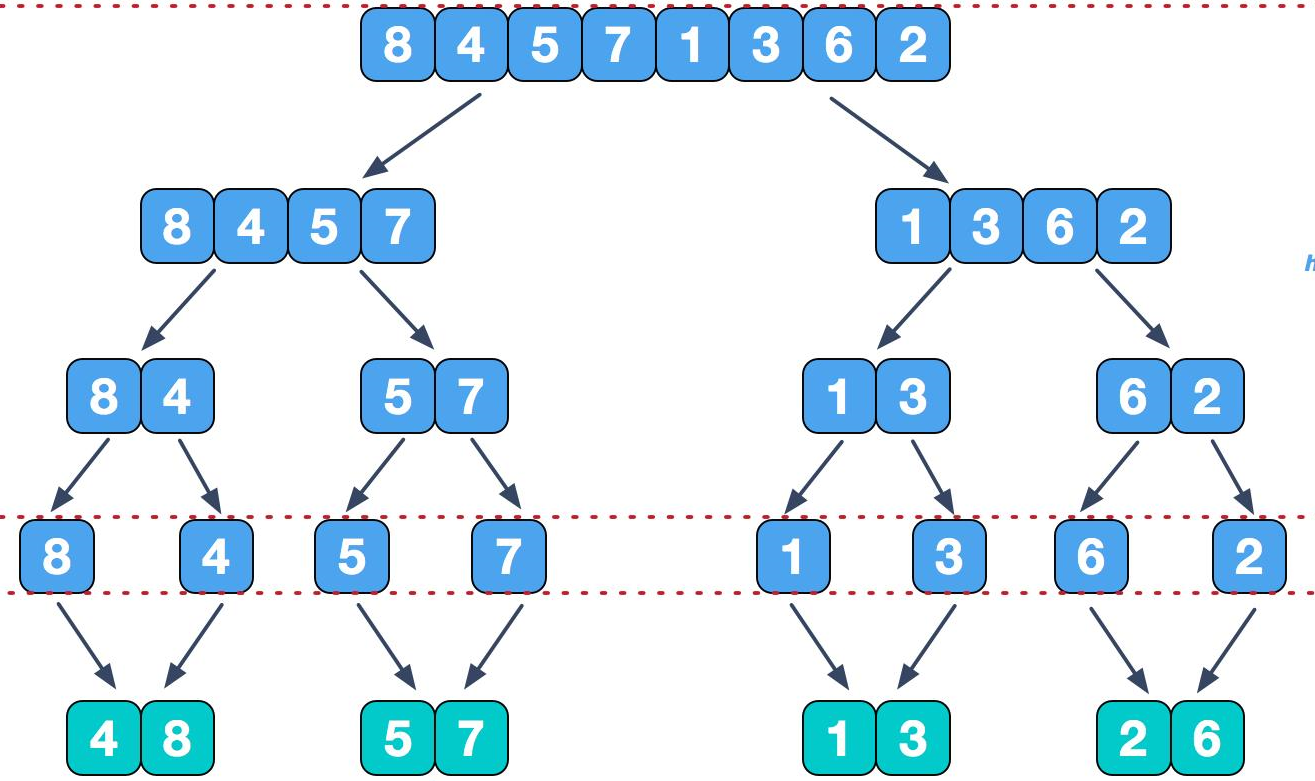
\includegraphics[scale=0.25]{images/4th_step.png}
    \end{center}
    Склеиваем:
    \begin{center}
        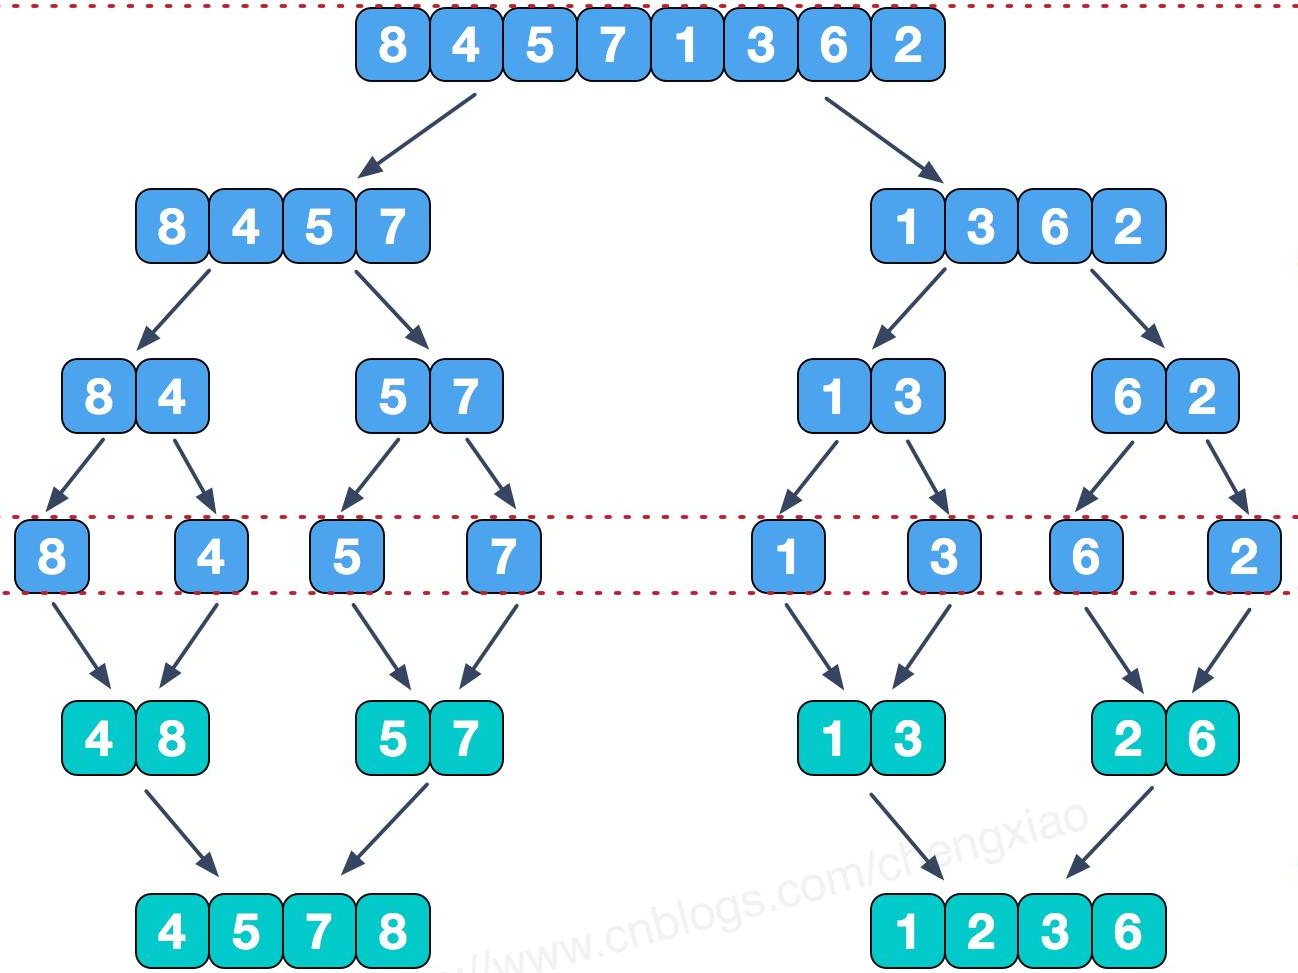
\includegraphics[scale=0.25]{images/5th_step.png}
    \end{center}
    Заводим два указателя на отсортированные части. Записываем минимальное из элементов указателя и сдвигаем тот, который записали, повторяем:
    \begin{center}
        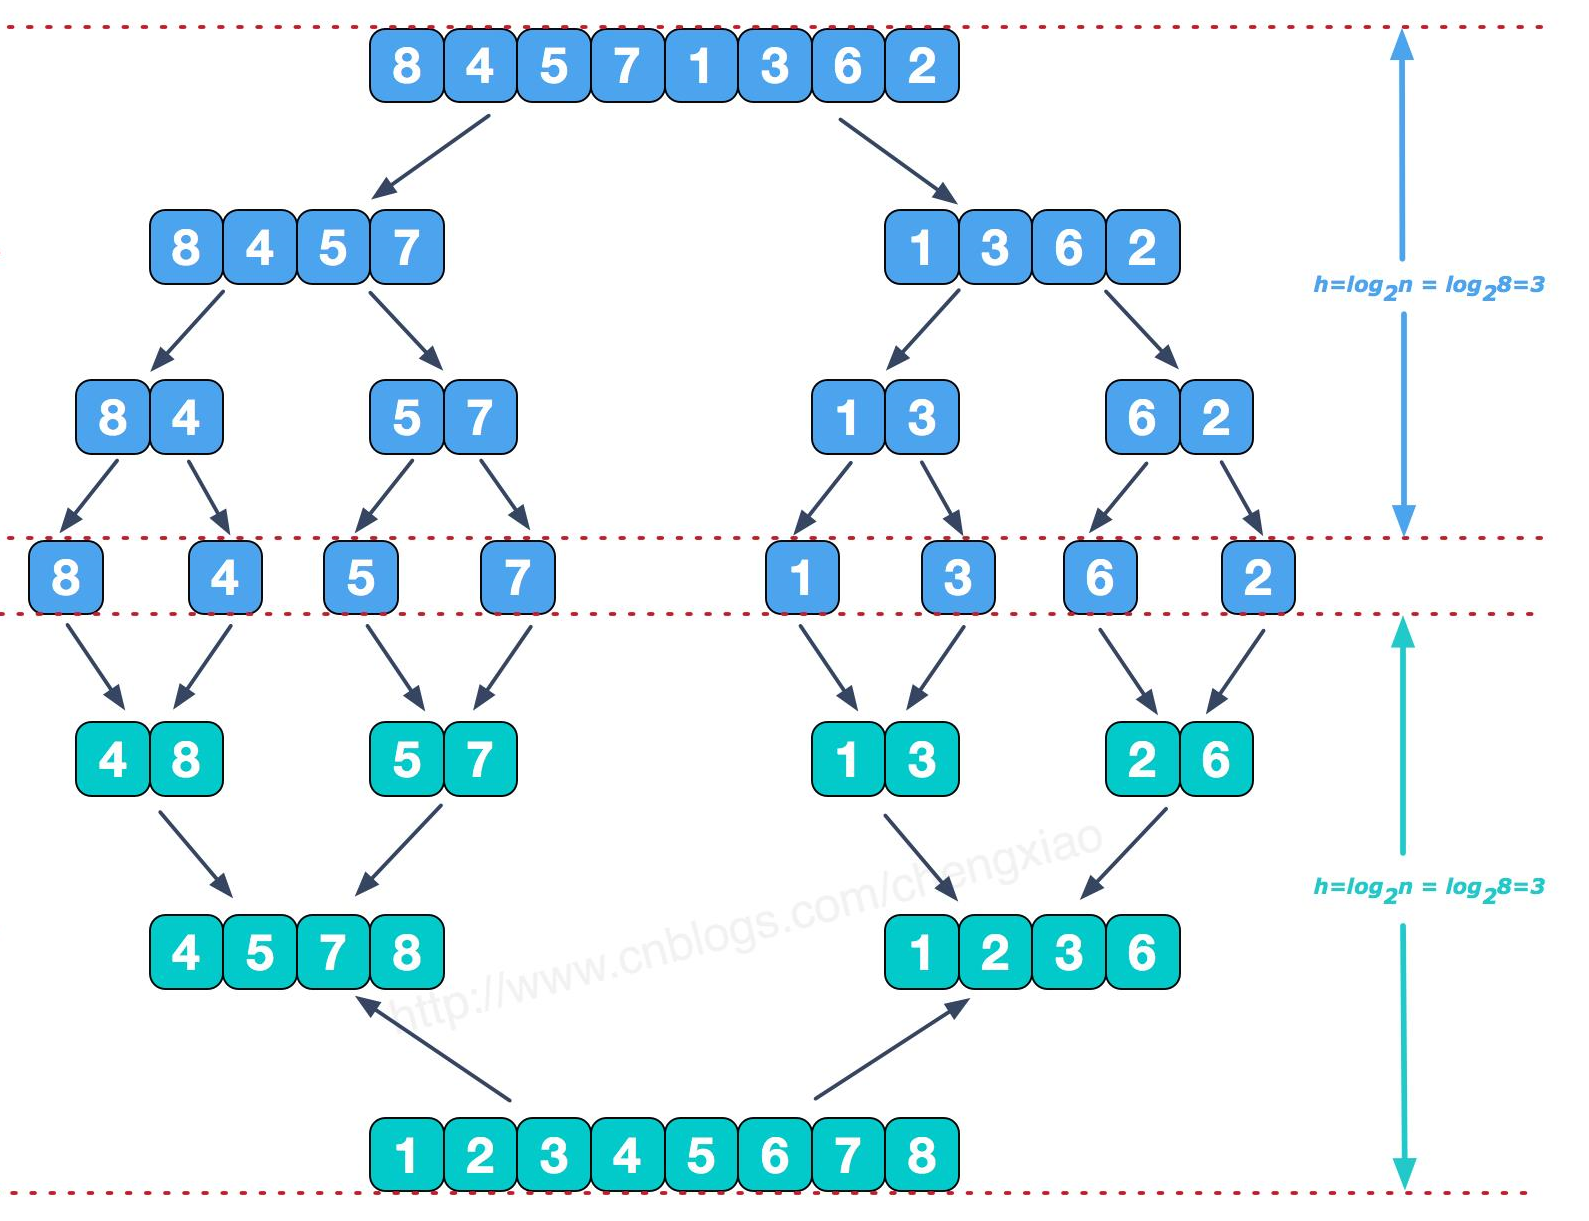
\includegraphics[scale=0.2]{images/Full.png}
    \end{center}
    Псевдокод:
    \begin{algorithmic}[1]
        \Function{MergeSort}{A}
        \If len(A) == 1 
        \State \Return
        \EndIf
        \State B, C -- две половины A
        \State MergeSort(B)
        \State MergeSort(C)
        \State Merge(B,C,A)
        \EndFunction
        \Function{Merge}{B,C,A}
        \State i=0, j=0, p=0
        \Repeat  
        \If (B[i] < C[j])
        \State A[p++] = B[i]
        \State ++i
        \Else
        \State A[p++] = C[j]
        \State ++j
        \EndIf
        \Until (i < len(B) and j < len(C))
        \Repeat 
        \State A[p++] = B[i]
        \State ++i
        \Until (i < len(B))
        \Repeat 
        \State A[p++] = C[j]
        \State ++j
        \Until (j < len(C))
        \EndFunction
    \end{algorithmic}
    \subsubsection*{Количество инверсий}
    Неотсортированный массив $a_1, \ldots, a_n$. Инверсия $(i, j): \ i < j, \ a_i > a_j$. Пусть $f(A)$ -- число инверсий в массиве $A$. $f(A) = f(B) + f(C) + $ количество инверсий, пересекающих разделитель. В момент, когда выбирается $B[i]$ все числа, стоящие слева от $B[i]$ его меньше, причем там ровно $j$ элементов из $C$. К ответу добавить $j$.
    \subsubsection*{Нерекурсивная реализация MergeSort}
    Будем считать, что $n$ -- степень двойки. (Если нет, то добавим слева или справа меньшие или большие, соответственно элементы, чем остальные в массиве. После сортировки их выкинем)
    \begin{algorithmic}[1]
        \Function{MergeSort}{a}
        \State queue<vector<int>> q
        \For{(int i = 0; i < n; ++i)}
        \State q.push({a[i]})
        \EndFor
        \While{(q.size() > 1)}
        \State vector<int> a = q.front()
        \State q.pop()
        \State vector<int> b = q.front()
        \State q.pop()
        \State q.push(Merge(a,b))
        \EndWhile
        \EndFunction
    \end{algorithmic}
    Ответ: $q.front()$. Время: $\bigOO(n\log n)$, Память: $\bigOO(n)$
    \subsection*{Быстрая сортировка (Quick sort)}
    Массив чисел: $a_1, \ldots, a_n$. Пусть $x$ -- случайный элемент массива. $Partition(A, x)$ -- перемешивание массива в виде: 
    \[
    \underbrace{[\hspace*{0.2cm} < x \hspace*{0.2cm}]}_{\substack{Quick\\Sort}}[\hspace*{0.2cm} = x \hspace*{0.2cm}] \underbrace{[\hspace*{0.2cm} > x \hspace*{0.2cm}]}_{\substack{Quick\\Sort}}
    \]
    Псевдокод
    \begin{algorithmic}[1]
        \Function{QuickSort}{A}
        \If (len(A) == 1)
        \State \Return
        \EndIf
        \State x -- случайный элемент $A$
        \State Partition(A,x)
        \State B -- числа <= x, C -- числа > x
        \State QuickSort(B)
        \State QuickSort(C)
        \EndFunction
    \end{algorithmic}
    В худшем случае: $\Omega(n^2)$.
    \begin{theorema}{}{}
        Математическим ожиданием времени работы на массиве длины $n$ есть $\Theta(n\log n)$.
    \end{theorema}
    \subsection*{Сортировка вставками (InsertSort)}
    Псевдокод 
    \begin{algorithmic}[1]
        \Function{InsertSort}{a}
        \If (len(A) == 1)
        \State \Return
        \EndIf
        \For{(i=1; i < n; ++i)}
        \State j = i-1
        \While{(j >= 0 and a[j] > a[j+1])}
        \State swap(a[j], a[j+1])
        \State --j
        \EndWhile
        \EndFor
        \EndFunction
    \end{algorithmic}
    Худший случай -- массив отсортирован в обратном порядке. Сложность $\bigOO(n^2)$
    \begin{center}
        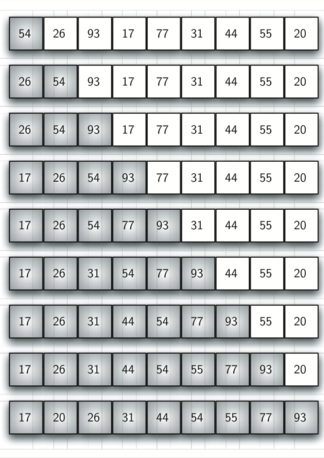
\includegraphics[scale=1.2]{images/insertsort.png}
    \end{center}
    \subsection*{Сортировка пузырьком (BubbleSort)}
    Псевдокод
    \begin{algorithmic}[1]
        \Function{BubbleSort}{a}
        \For{(int i = 0; i < n-2; ++i)}
        \For{(int j = 0; j < n-2; ++j)}
        \If a[j] > a[j+1]
        \State swap(a[j], a[j+1])
        \EndIf
        \EndFor
        \EndFor
        \EndFunction
    \end{algorithmic}
    Сложность: $\bigOO(n^2)$
    \subsubsection*{Оптимизация}
    \begin{enumerate*}
        \item После $i$ итераций, в конце $i$ чисел отсортировано;
        \begin{algorithmic}[1]
            \Function{BubbleSort}{a}
            \For{(int i = 0; i < n-2; ++i)}
            \For{(int j = 0; j < n-i-2; ++j)}
            \If a[j] > a[j+1]
            \State swap(a[j], a[j+1])
            \EndIf
            \EndFor
            \EndFor
            \EndFunction
        \end{algorithmic}
        \item Если не было $swap$, то массив уже отсортирован.
        \begin{algorithmic}[1]
            \Function{BubbleSort}{a}
            \State i=0
            \State isSwapped=True
            \While{isSwapped}
            \State isSwapped=False
            \For{(int j = 0; j < n-i-2; ++j)}
            \If{a[j] > a[j+1]}
            \State swap(a[j], a[j+1])
            \State isSwapped = True
            \EndIf
            \EndFor
            \State ++i
            \EndWhile
            \EndFunction
        \end{algorithmic}
    \end{enumerate*}

    \section{Представление матриц и векторов. Алгоритмы умножения матриц и эффективные
    способы их реализации. Численные методы решения систем линейных уравнений.}
    Векторы -- массивы двух типов. Статические массивы -- структуры фиксированного размера. Динамические -- размер можно менять в процессе выполнения программы. В $c++$ -- $std::vector$. Позволяет эффективно добавлять элементы в конце и удалять последние элементы.
    \begin{lstlisting}
        std::vector<int> v = {2,4,3};
        v.push_back(3); // [2,4,3,3]
        v.push_back(5); // [2,4,3,5]
        std::cout << v.back() << "\n"; // 5
        v.pop_back(); // [2,4,3]
    \end{lstlisting}
    Вектор -- частный случай матрицы размера $n\times 1$, где $n$ -- длина вектора. Итого: матрица представляет собой двумерный массив (вектор векторов). Операции над матрицами в линейной алгебре. Умножение двух двух матриц за время $O(n^3)$:
    \begin{lstlisting}
        for (int i = 1; i <= n; ++i) {
            for (int j = 1; j <= n; ++j) {
                for (int k = 1; k <= n; ++k) {
                    ans[i][j] += a[i][k]*b[k][j];
                }
            }
        }
    \end{lstlisting} 
    Возведение в степень матрицы считается также, как и для возведения числа:
    \[
        A^n = \left\{\begin{array}{c}
            A \cdot A^{n-1}, \ \text{ если $n$ -- четное}\\
            \left(A^{1/2}\right)^2, \ \text{ если $n$ четное}.              
        \end{array}
            \right.  
    \]  
    Время: $\bigOO(k^3 \log n)$. $k$ -- размерность квадратной матрицы, $n$ -- степень
    \subsection*{Методы решения СЛАУ}
    \subsubsection*{Метод Гаусса}
    Система уравнений имеет хорошую плотность и среднюю обусловленность:
    \[
        Ax = b.  
    \]
    За счет элементарных преобразования над строками (см. Линейная алгебра) матрица СЛАУ преобразуется в верхнюю (или нижнюю) треугольную -- прямой ход метода. Обратный ход метода -- определяются неизвестные. 
    \par 
    \textbf{Прямой ход.} На первом шаге алгоритма выберем диагональный элемент в качестве главного (pivot), причем такой, чтобы он не был равен нулю (если равен, то меняем строки местами), строку и столбец, на пересечении которых стоит pivot, объявим ведущими. Обнулим элементы ведущего столбца. В результате повторения для каждого столбца (2-й шаг -- pivot $= a^{1}_{22}$). В результате прямого ходя получим верхнетреугольную матрицу вида:
    \[
        \begin{bmatrix}
            a_{11} & a_{12} & a_{13} & \ldots & a_{1n} &  \dashline b_1\\
            0 & a_{22}^1 & a_{23}^1 & \ldots & a_{2n}^1 & \dashline b_2\\
            0 & 0 & a_{33}^2 & \ldots & a_{3n}^2 & \dashline b_3\\
            \ldots & \ldots & \ldots & \ldots & \ldots & \dashline \ldots \\
            0 & 0 & 0 & \ldots & a_{nn}^{n-1} & \dashline b_n^{n-1}
        \end{bmatrix}
    \]  
    В обратном ходе алгоритма выражаем итеративно в обратном порядке значения решения:
    \[
        \left\{\begin{array}{ll}
            a_{nn}^{n-1}x_n = b_n^{n-1} & \Longrightarrow x_n\\
            a_{n-1}^{n-2}x_{n-1} + a_{n-1}^{n-2}x_n = b_{n-1}^{n-2} & \Longrightarrow x_{n-1}\\
            \hdash & \hdash\\
            a_{11}x_1 + \ldots + a_{1n}x_n = b_1 & \Longrightarrow x_1.
        \end{array}\right.
    \]
    \begin{note}{}{}
        Условия совместности системы (теорема Кронекера-Капелли) никто не отменял
    \end{note}
    \begin{note}{}{}
        Так же при таком методе возможно получения определителя, но надо хранить информацию о перестановке строк (определитель меняет знак):
        \[
            \det A = a_{11}a^1_{22}\ldots a_{nn}^{n-1}.  
        \]
    \end{note}
    Сложность алгоритма: $\bigOO(n^3)$.
    \subsubsection*{Метод прогонки}
    Метод прогонки эффективен, но работает только для матриц с трехдиагональной структурой. Является частным случаем метода Гаусса.
    Пусть СЛУ имеет вид:
    \[
    \left\{
        \begin{array}{l}
            b_1 x_1 +  c_1 x_2  = d_1,\\
            a_2 x_1 +  b_2x_2+c_2x_3  =d_2,\\
            \hspace*{1cm} a_3x_2 + b_3x_3 + c_3 x+4 = d_3,\\
            \hdash \\
            \hspace*{1cm} a_{n-1} x_{n-2} + b_{n-1}x_{n-1} + c_{n-1}x_n = d_{n-1}\\
            \hspace*{2.5cm} a_{n}x_{n-1} + b_nx_n = d_n, \ c_n = 0
        \end{array}
    \right.    
    \]
    Решение ищем в виде:
    \[
        x_i = A_{i}x_{i+1} + B_i,
    \] 
    где $A_i, \ B_i$ -- прогоночные коэффициенты, подлежащие определению. Чтобы их выразить:
    \[
        x_1 = \dfrac{-c_1}{b_1}x_2 + \dfrac{d_1}{b_1} = A_1 x_2 + B_1
    \]
    Тогда
    \[
        A_1 = \dfrac{-c_1}{b_1}, \ B_1 = \dfrac{d_1}{b_1}.  
    \]
    Из второго уравнению аналогично выразим $x_2$ через $x_3$:
    \[
        x_2 = \dfrac{-c_2}{b_2 + a_2A_1} x_3 + \dfrac{d_2 - a_2B_1}{b_2 + a_2 A_1} = A_2 x_3 + B_2,
    \]
    откуда
    \[
        A_2 = \dfrac{-c_2}{b_2+a_2A_1}, \ B_2 = \dfrac{d_2 - a_2B_1}{b_2 + a_2A_1}.  
    \]
    Тогда 
    \[
        x_i = \dfrac{-c_i}{b_i + a_i A_{i-1}} x_{i+1} + \dfrac{d_i - a_i B_{i-1}}{b_i+a_iA_{i-1}},  
    \]
    следовательно:
    \[
        A_{i} = \dfrac{-c_i}{b_i + a_iA_{i-1}}, \ B_{i} = \dfrac{d_i - a_iB_{i-1}}{b_i + a_iA_{i-1}}.  
    \]
    Из последнего уравнения СЛУ:
    \[
        x_n = \dfrac{-c_n}{b_n + a_n A_{n-1}} x_{n+1} + \dfrac{d_n-a_nB_{n-1}}{b_n + a_nA_{n-1}} = 0 \cdot x_{n+1} + B_n, 
    \]
    то есть
    \[
        A_n = 0\ (c_n = 0), \hspace*{0.5cm} B_n = \dfrac{d_n-a_nB_{n-1}}{b_n+a_nA_{n-1}} = x_n  
    \]
    В результате прогоночные коэффициенты вычисляются следующим образом:
    \[
        A_i = \dfrac{-c_i}{b_i + a_i A_{i-1}}, \ B_{i} = \dfrac{d_i - a_i B_{i-1}}{b_i + a_i A_{i-1}}, \hspace*{0.2cm} i = \overline{2, n-1}
    \]
    Причем (из-за того, что $a_1 = 0$)
    \[
        A_{1} = \dfrac{-c_1}{b_1}, \ B_1 = \dfrac{d_1}{b_1}  
    \]
    И так как $c_n = 0$:
    \[
        A_n = 0, \hspace*{0.5cm} B_n = \dfrac{d_n-a_nB_{n-1}}{b_n + a_nA_{n-1}}.  
    \]
    Обратный ход метода прогонки:
    \[
        \left\{
            \begin{array}{l}
                x_n = A_nx_{n+1} + B_n = B_n,\\
                x_{n-1} = A_{n-1}x_n + B_{n-1},\\
                x_{n-2} = A_{n-2}x_{n-1} + B_{n-2},\\
                \hdash\\
                x_1 = A_1 x_2 + B_1.
            \end{array}
        \right.  
    \]
    Алгоритмическая сложность: $\bigOO(8n+1) = \bigOO(n)$.
    \subsection*{Итерационные методы решения СЛУ}
    Используются при большом количестве уравнений обычные методы труднореализуемы. Методы последовательных приближений, в которых в последующих вычислениях используются предыдущие называются итерационными. 
    \subsubsection*{Метод простых итераций}
    Рассмотрим СЛУ:
    \[
      \left\{
        \begin{array}{l}
            a_{11}\underline{x}_1 + a_{12}x_2 + \ldots + a_{1n}x_n = b_1,\\
            a_{21}x_1 + a_{22}\underline{x}_{2} + \ldots + a_{2n}x_n = b_2,\\
            \hdash\\
            a_{n1} x_1 + a_{n2}x_2 + \ldots + a_{nn}\underline{x}_n = b_n
        \end{array}
        \right.  
    \]
    с невырожденной матрицей $A$. Представим в виде:
    \[
        x = \beta + \alpha x,
    \]
    где 
    \[
        x = \begin{bmatrix}
            x_1 \\
            \vdots \\
            x_n
        \end{bmatrix}, \hspace*{0.5cm} \beta = \begin{bmatrix}
            \beta_1 \\
            \vdots\\
            \beta_n
        \end{bmatrix}, \hspace*{0.5cm} \alpha = \begin{bmatrix}
            \alpha_{11} & \ldots & \alpha_{1n}\\
            \vdots & \ddots & \vdots \\
            \alpha_{n1} & \ldots & \alpha_{nn}
        \end{bmatrix}.
    \]
    Разрешим первую систему относительно подчеркнутых неизвестных при ненулевых диагональных элементах (если равен -- меняем местами). Получим выражения 
    \[
        \beta_i = \dfrac{b_i}{a_{ii}}; \hspace*{0.5cm} \alpha_{ij} = \left\{ \begin{array}{l}
            -\dfrac{a_{ij}}{a_{ii}}, \ i, j = \overline{1, n}, \ i \neq j;\\
            0, \hspace*{0.5cm} i = j,\ i = \overline{1,n}.
        \end{array} \right.  
    \]
    В качестве нулевого приближения выберем $x^{(0)} = \beta$, или \mbox{$\left(x_1^{(0)}\ x_2^{(0)}\ \ldots \ x_n^{(0)}\right)^\intercal = (\beta_1\ \beta_2 \ \ldots \ \beta_n )$}. Тогда метод простых итераций -- последовательные вычисления вида:
    \[
        \left\{
            \begin{array}{l}
                x^{(0)} = \beta,\\
                x^{(1)} = \beta + \alpha x^{(0)},\\
                x^{(2)} = \beta + \alpha x^{(1)},\\
                \hdash \\
                x^{(k)} = \beta + \alpha x^{(k-1)}.
            \end{array}
         \right.  
    \]
    \begin{theorema}{(О сходимости МПИ)}{}
        Метод простых итераций сходится к единственному решению СЛУ при любом начальном приближении $x^{(0)}$, если какая-либо норма матрицы $\alpha$ эквивалентной системы меньше 1:
        \[
            ||\alpha|| < 1\ \forall ||\alpha || \text{ и } \forall x^{(0)}.  
        \]
    \end{theorema}
    \subsubsection*{Метод Зейделя}
    Метод простых итераций медленно сходится, для ускорения существует метод Зейделя. Идея заключается в том, что при вычислении компонента $x_i^{(k+1)}$ вектора неизвестных на $(k+1)$-й итерации используются значения $x_1^{(k+1)}, \ldots, x_{i-1}^{(k+1)}$, уже вычисленные. Значения остальных $x_{i}^{(k)}, \ldots, x_{n}^{(k)}$ из предыдущей итерации. Как и в МПИ \mbox{$x^{(0)} = (\beta_1 \ \beta_2 \ \ldots \ \beta_n)^\intercal$}. Тогда метод Зейделя для известного вектора $\left(x_1^{(k)} \ x_2^{(k)} \ \ldots \ x_{n}^{(k)}\right)^\intercal$ на $k$-ой итерации будет иметь вид:
    \[
        \left\{
            \begin{array}{l}
                x_1^{(k+1)} = \beta_1 + \alpha_{11}x_1^{(k)} + \alpha_{12}x_2^{(k)} + \ldots + \alpha_{1n}x_n^{(k)},\\
                x_2^{(k+1)} = \beta_2 + \alpha_{21}x_1^{(k+1)} + \alpha_{22}x_2^{(k)} + \ldots + \alpha_{2n}x_n^{(k)},\\
                x_3^{(k+1)} = \beta_3 + \alpha_{31}x_1^{(k+1)} + \alpha_{32}x_2^{(k+1)} + \ldots + \alpha_{3n}x_n^{(k)}, \\
                \hdash\\
                x_n^{(k+1)} = \beta_n + \alpha_{n1}x_1^{(k+1)} + \alpha_{n2}x_2^{(k+1)} + \ldots + \alpha_{nn}x_n^{(k)}
            \end{array}
        \right.
    \]
    Можно заметить $x^{(k+1)} = \beta + Bx^{(k+1)} + Cx^{(k)}$, где $B$ -- нижняя треугольная матрица с диагональными элементами, равными 0, а $С$ -- верхнетреугольная с диагональными элементами, не равными нулю. $\alpha = B + C$. Итого:
    \[
            x^{(k+1)} = (E-B)^{-1}Cx^{(k)} + (E-B)^{-1}\beta.
    \]
    Таким образом, метод Зейделя -- МПИ с матрицей правых частей $\alpha = (E-B)^{-1}C$ и вектором правых частей $\beta = (E-B)^{-1}\beta.$
    \section{Численное дифференцирование и интегрирование. Численные методы для решения
    систем дифференциальных уравнений.}

    \section{Граф. Ориентированный граф. Представления графа. Обход графа в глубину и в ширину.
    Топологическая сортировка. Подсчет числа путей в орграфе.}
    Дадим определения графа и ориентированного графа.
    \begin{definition}{(Неориентированный граф)}{}
        Пара $G= (V,E)$, где $V$ -- множество, $E \subset C_V^2$ (множество упорядоченных пар)
    \end{definition}
    \begin{definition}{(Ориентированный граф)}{}
        Ориентированный граф $G= (V,E)$, $V$ -- множество, $E\subset V\times V$
    \end{definition}
    \begin{definition}{(Путь)}{}
        Путь $v_1, v_2, \ldots v_k$ -- последовательность вершин таких, что $(v_1, v_2) \in E, \ (v_2, v_3) \in E, \ldots , (v_{k-1}, v_{k}) \in E$.
    \end{definition}
    Путь называется реберно простым, если ребра в нем не повторяются. Путь называется вершинно простым, если вершины в нем не повторяются. \vspace*{0.5cm}

    \begin{note}{}{}
        Из вершинной простоты следует реберная.
    \end{note} 
    \begin{definition}{(Цикл)}{}
        Путь $v_1, \ldots, v_k$ называется циклом, если $v_1 = v_k.$
    \end{definition}
    \begin{note}{}{}
        Определения реберной и вершинной простоты наследуются.
    \end{note}
    \begin{definition}{(Достижимость)}{}
        Из вершины $u$ достижима вершина $v$, если существует путь $v_1, \ldots, v_k:\ v_1 = u, \ v_k = v.$
    \end{definition}
    \begin{definition}{(Связность)}{}
        Если $G$ -- неориентированный граф, то отношение связности: 
        \[
            u\sim v,  
        \]
        если из $u$ есть путь в $v$.
    \end{definition}
    \begin{note}{}{}
        Отношение связности в неориентированном графе -- отношение эквивалентности.
    \end{note}
    \begin{definition}{}{}
        Классы эквивалентности по отношению связности -- компоненты связности.
    \end{definition}
    \begin{definition}{}{}
        Если $G$ -- ориентированный граф, то введем отношение сильной связности:
        \[
            u\sim v,
        \]
        если $\exists$ путь из $u$ в $v$ и $\exists$ путь из $v$ в $u$.
    \end{definition}
    \begin{note}{}{}
        $\sigma$ -- отношение эквивалентности.
    \end{note}
    \begin{definition}{(Комп-нты сильной связности)}{}
        Компоненты сильной связности -- классы эквивалентности по отношению сильной связности.
    \end{definition}
    \subsection*{Хранение графов}
    \subsubsection*{Матрица смежности}
    \[
        M_{ij} = \left\{ 
            \begin{array}{l}
                1, \text{ если } (i,j) \in E\\
                0, \text{ иначе }.
            \end{array}
        \right.
    \]
    \begin{itemize}
        \item[+] за $\bigOO(1)$ проверка наличия ребра;
        \item[-]  требует $\Omega(n^2)$ памяти.
    \end{itemize}
    \subsubsection*{Список ребер}
    \[
        \begin{array}{l}
            u_1, v_1\\ 
            u_2, v_2\\
            \vdots\\
            u_m, v_m           
        \end{array}
    \]
    \begin{itemize}
        \item[+] естественность;
        \item[-] неудобство обработки. 
    \end{itemize}
    \subsubsection*{Список смежности}
    \useshortskip
    \[
        \begin{array}{c}
            l_1\\
            \vdots\\
            l_n
        \end{array} \hspace*{0.5cm} l_u = \{v: \ (u, v) \in E\}
    \]
    \begin{itemize}
        \item[+] требует $\bigOO(n+m)$ памяти;
        \item[+] для каждой вершины знаем множество соседей;
        \item[-] за $\bigOO(1)$ нельзя проверить наличие ядра в графе.  
    \end{itemize}
    \subsection*{DFS}
    \begin{lstlisting}
        std::vector<std::vector<int>> g;
        std::vector<int> tin, tout;
        int timer = 0;
        std::vector<string> color; // WHITE
        vector<int> parent;
        void dfs(int v, int p = -1) {
            tin[v] = timer++;
            parent[v] = p;
            color[v] = GRAY; // GRAY -- IN WORK
            for (int to: g[v]) {
                if (color[to] != WHITE) 
                    continue;
                dfs(to, v);
            }
            tout[v] = timer++;
            color[v] = BLACK; // the end
        }
    \end{lstlisting}
    \begin{lemma}{(о белых путях)}{}
        Если в момент $tin[v]$ есть некий путь из $v$ по белым вершинам, то к моменту $tout[v]$ все вершины этого пути будут черными.
    \end{lemma}
    \cons Если запустить $dfs(s)$, то алгоритм посетит те и только те вершины, которые были достижимы из s.
    \par
    \cons Пусть в $main$ выполняется $dfs(s)$. Тогда в графе $\exists$ цикл, достижимый из $S \Leftrightarrow \ dfs$ когда-то находит ребро в серую вершину.  \vspace*{0.5cm}

    \begin{note}{}{}
        Таким образом проверяется только наличие цикла.
    \end{note}
    \begin{note}{}{}
        Чтобы найти сам цикл надо использовать массив $parent$.
    \end{note}
    \subsection*{Топологическая сортировка}
    \begin{definition}{(Топологическая сортировка)}{}
        $DAG$ -- directed acyclic graph (ориентированный ациклический граф). Топологическая сортировка $p_1, \ldots, p_n$ -- перестановка вершин графа, такая что ребра графа ведут только слева направо: $p_i \to p_j$.
    \end{definition}
    Найдем топологическую сортировку в $DAG$.
    \begin{lstlisting}{1}
        for (v = 0; v < n-1) {
            if (color[v] == "WHITE") dfs(v);
        }
    \end{lstlisting}
    Вывести все вершины в порядке убывания tout.
    \par
    \myexe{Найти число путей в $DAG$.}
    Сначала топсорт. Пусть $dp[v]$ -- число путей, начинающихся в $v$:
    \[
        dp[v] = 1 + \sum\limits_{\substack{u:\\(v,u)\in E}} dp[u]. 
    \]
    Проход справа-налево. Сложность $\bigOO(n + m)$.
    \subsection*{Алгоритм Косарайю}
    Нахождение компонент сильной связности.
    \par
    Пусть $p$ -- список вершин в порядке убывания $tout$. Красим всё в белый, проходим по $p$, запускаем $dfs\ R$ от белых вершин. Всё, что посещает $dfs$ -- очередная компонента сильной связности.
    \section{Алгоритмы поиска кратчайших путей в графе. Алгоритм Дейкстры. Алгоритм Форда-
    Беллмана. Алгоритм Флойда. Алгоритм A*.}
    \columnbreak
    \section{Недетерминированные конечные автоматы, различные варианты определения.
    Детерминированные конечные автоматы. Их эквивалентность. Машина Тьюринга.}
\end{multicols}